


\eat
{

\begin{figure*}[t]
\begin{minipage}[b]{0.31\linewidth}
\begin{center}
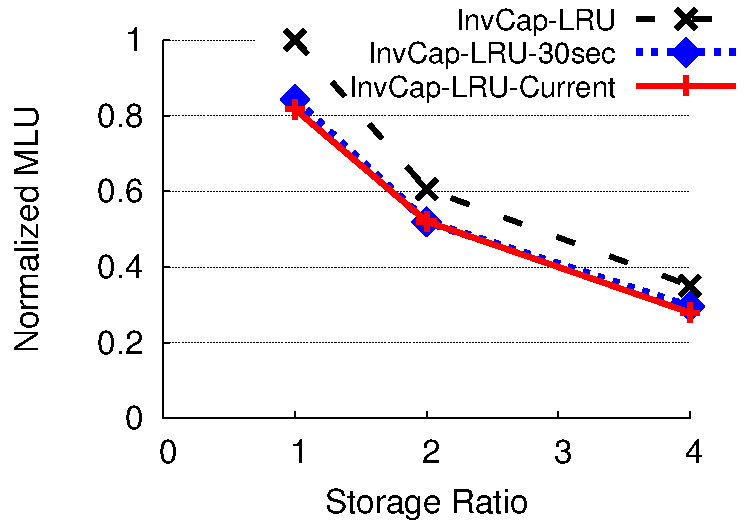
\includegraphics[width=\textwidth]{graphSet1/lrusnmp/ATTVideos.pdf}
\end{center}
\vspace{-0.25in}
\caption{Link utilization aware request redirection helps \invlru\ reduce network cost up to 21\%. Entertainment trace, US-ISP}
\label{fig:lrusnmp}
\end{minipage}
\vspace{-0.2in}
\hspace{0.3cm}
\begin{minipage}[b]{0.31\linewidth}
\begin{center}
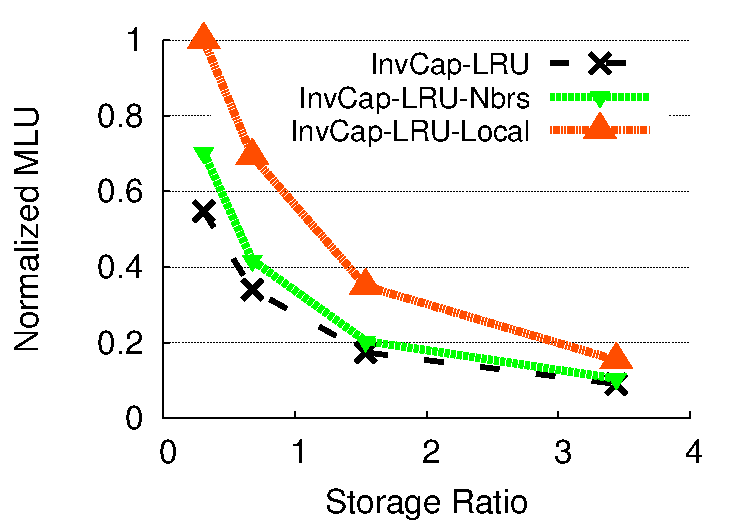
\includegraphics[width=\textwidth]{graphSet1/lrulocalnew/AbileneDownloads.pdf}
\end{center}
\vspace{-0.25in}
\caption{\textsf{\invlru-Nbrs} and \textsf{\invlru-Local} have 27\% and 100\% higher network cost than \invlru. Downloads trace, Abilene}
\label{fig:lrulocalnew}
\end{minipage}
\hspace{0.3cm}
\begin{minipage}[b]{0.31\linewidth}
\begin{center}
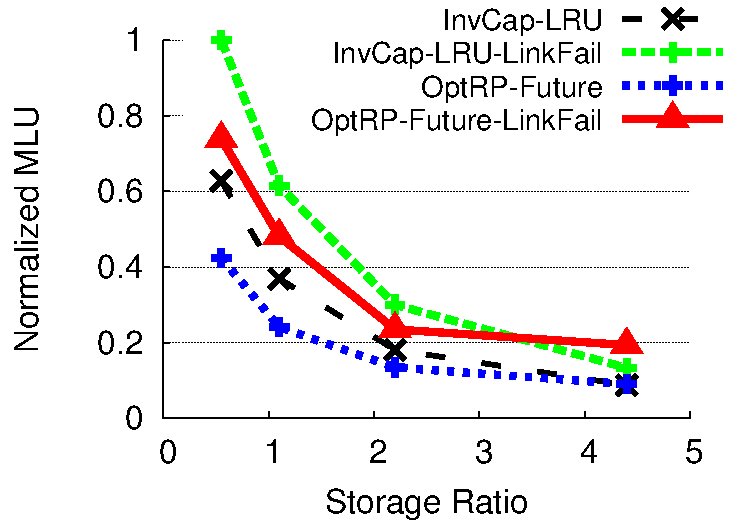
\includegraphics[width=\textwidth]{graphSet1/linkfailurecompare/AbileneVideos.pdf}
\end{center}
\vspace{-0.25in}
\caption{During link failures, \invlru\ can achieve a lower network cost than \optrpfuture\ at high storage ratios. Entertainment trace, Abilene}
\label{fig:linkfailurecompare}
\end{minipage}
\end{figure*}
}


\subsubsection{Content chunking}
\label{sec:chunking}
Content chunking is widely used today to improve content delivery and common protocols  such as HTTP \cite{rfc2616} and Apple HLS  \cite{applehls} support content chunking.
This experiment analyzes the effect of content chunking on our findings.  In these experiments, we split videos into chunks of 5 minute duration. The size of a video chunk depends on the video bitrate.  For the downloads trace, we split content into chunks of size 50 MB.

%In Figure \ref{fig:chunking}, we compare performance of \invlru\ and \optrpfuture\ with and without chunking.  

Our results show that  although chunking improves performance of both \invlru\ and \optrpfuture, it significantly improves the performance of \invlru\ relative to \optrpfuture\ (see Figure \ref{fig:chunking}).  Due to chunking, the maximum difference between the MLU of  \invlru\ and \optrpfuture\ reduces from 2.5$\times$ to 1.4$\times$. At the maximum storage ratio, \invlru\ is at most 18\% worse compared to \optrpfuture. Our experiments on other traces and topologies (omitted for brevity)  show that \invlru\ has at most 4\% higher network cost than \optrpfuture\ at the maximum storage ratio. An exception is  the news trace, where chunking makes a small difference as  more than 95\% content is of duration less than our chunk size.  Hence, chunking strengthens our conclusion that \invlru\ achieves close to the best possible network cost for an NCDN. Even with chunking,  \optrp\ has up to 7$\times$ higher MLU compared to \invlru\ (not shown in Figure \ref{fig:chunking}). This is because chunking does not help \optrp's primary problem of not being able to adapt effectively to new content, so it continues to incur a high cost.



\begin{figure*}
\begin{minipage}[b]{0.31\linewidth}
\begin{center}
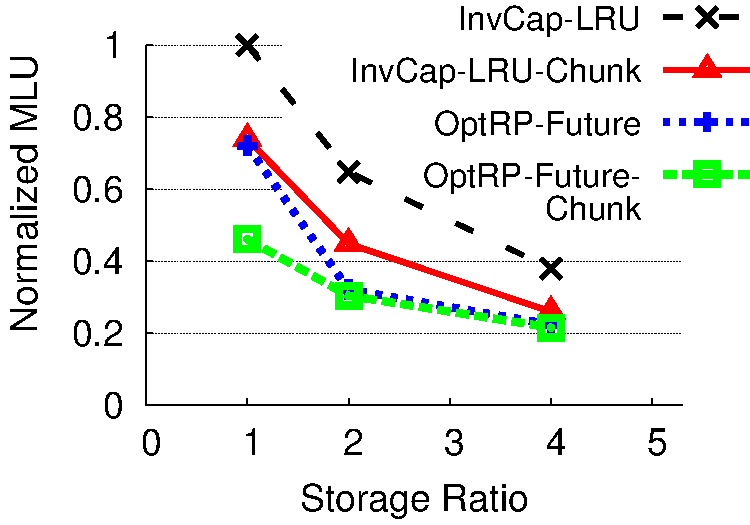
\includegraphics[width=\textwidth]{graphSet1/chunkcomp/ATTVideos.pdf}
\end{center}
\vspace{-0.25in}
\caption{[Entertainment, US-ISP] Content chunking helps bridge the gap between \invlru\ and \optrpfuture.}
\label{fig:chunking}
\end{minipage}
\vspace{-0.15in}
\hspace{0.2cm}
\begin{minipage}[b]{0.31\linewidth}
\begin{center}
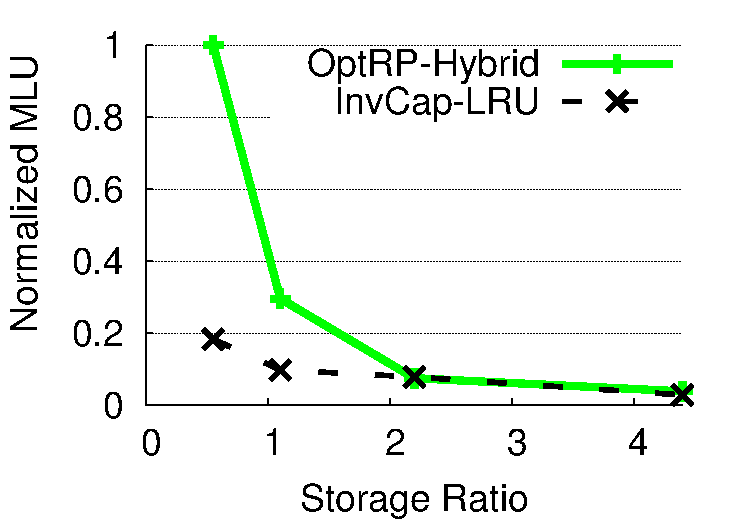
\includegraphics[width=\textwidth]{graphSet1/hybrid/AbileneVideos.pdf}
\end{center}
\vspace{-0.25in}
\caption{[Entertainment, Abilene] Hybrid placement schemes perform at best as well as \invlru.}
\label{fig:hybrid}
\end{minipage}
\hspace{0.2cm}
\begin{minipage}[b]{0.31\linewidth}
\begin{center}
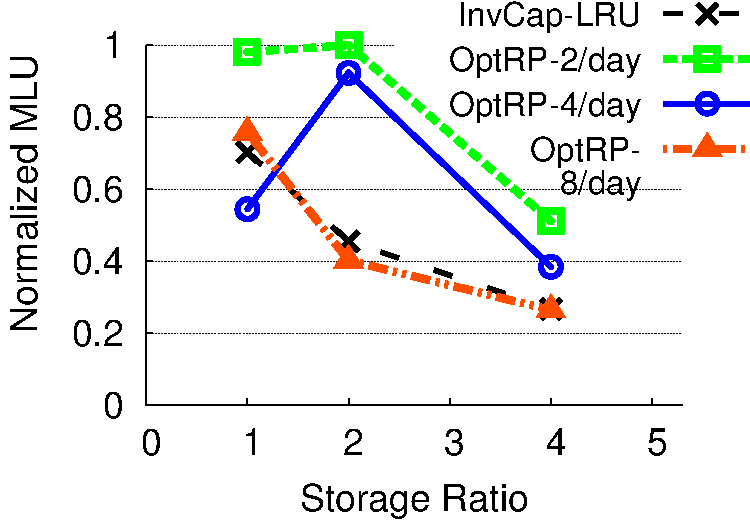
\includegraphics[width=\textwidth]{graphSet1/tefrequency/ATTVideos.pdf}
\end{center}
\vspace{-0.25in}
\caption{[Entertainment, US-ISP] \optrp\ does not outperform  \invlru\ despite engineering  8 times a day.}
\label{fig:optrpfrequency}
\end{minipage}
\end{figure*}


%In Figure \ref{fig:chunking}, we compare performance of \invlru\ and \optrpfuture\ with and without chunking.  While chunking improves performance of both \invlru\ and \optrpfuture, it significantly improves the performance of \invlru\ relative to \optrpfuture. Due to chunking, the maximum difference between  \invlru\ and \optrpfuture\ reduces from 2.5$\times$ to 1.4$\times$, and at the maximum storage ratio, \invlru\ has less than 20\% higher MLU compared to \optrpfuture. We find qualitatively similar conclusions on experiments with other traces and topologies.  Hence, chunking strengthens our conclusion that \invlru\ achieves close to the best possible MLU for an NCDN. Even with chunking,  \optrp\ has up to 7$\times$ higher MLU compared to \invlru\ (not shown in Figure \ref{fig:chunking}). This is because chunking does not help \optrp's primary problem of not being able to adapt effectively to new content, so it continues to incur a high cost.

\subsubsection{Alternative \planned\  schemes}
\label{sec:hybrid}
%The experiments so far  suggest that a \planned\ scheme that engineers placement and routing once a day based on the previous day's demand performs poorly compared to a \unplanned\ scheme, \invlru. 

The experiments so far  suggest that a \planned\ scheme that engineers placement and routing once a day based on the previous day's demand performs poorly compared to a \unplanned\ scheme, \invlru. Therefore, in this section, we evaluate the performance of two alternative \planned\ schemes. 



First, we evaluate a hybrid placement scheme, which splits the storage at each node into two parts - one for a \planned\ placement based on the previous day's content demand (80\% of storage) and the other for placing the content in a \unplanned\ LRU manner (20\% of storage). This hybrid strategy is similar to that used in \cite{Applegate2010}. We find that \invlru\ performs either as well or better than the hybrid scheme.  We also experimented with assigning a greater fraction of storage to \unplanned\ placement (omitted for brevity), but the above conclusions remain unchanged in those experiments. Of course, a carefully designed hybrid scheme by definition should perform at least as well as the \unplanned\ and \planned\ schemes, both of which are extreme cases of a hybrid strategy. However, we were unable to design simple hybrid strategies that consistently outperformed fully \unplanned\ placement and routing.

\eat
{
Next, we analyze the performance of \planned\ schemes that engineer placement and routing multiple times each day at equal intervals - twice/day, 4 times/day, and 8 times/day. In all cases, we use the content demand in the past 24 hours to engineer placement and routing. As Figure \ref{fig:optrpfrequency} shows, \optrp\ needs to engineer 8 times/day to match the performance of a \unplanned\ placement. 
In other cases, \invlru\ performs better. Considering the effort of executing a \planned\ placement - measuring content demand at all PoPs, solving a time-consuming optimization problem, moving content to new locations - and the frequency at which it needs to be done (8 times/day)  even to match the simple \invlru\ scheme, further strengthens the case for a \unplanned\ placement. 
}
%Next, we analyze the performance of \optrp\ when it engineers placement and routing multiple times each day at equal intervals
Next, we analyze the performance of \planned\ schemes that engineer placement and routing multiple times each day at equal intervals - twice/day, 4 times/day, and 8 times/day. In all cases, we engineer using the content demand in the past 24 hours. As Figure \ref{fig:optrpfrequency} shows, \optrp\ needs to engineer 8 times/day to match the performance of the \invlru\ scheme. In all other cases, \invlru\ performs better.  In fact, the experiment shown here represents the best case for \optrp. Typically, \optrp\ performs worse even when engineering is done 8 times/day, e.g., on the news trace, we find \optrp\ incurs up to 4.5$\times$ higher MLU compared to \invlru\ even on engineering 8 times/day.


Executing a \planned\ placement requires considerable effort---measuring content matrix, solving a computationally intensive optimization, and moving content to new locations. Further, a \planned\ placement needs to be executed  8 times a day (or possibly more) even to match the cost achieved by a \unplanned\ strategy. Our position is that NCDNs are better served by opting for a much simpler \unplanned\ strategy and provisioning more storage, in which case, a \unplanned\ strategy  already obtains a network cost close to the best a \planned\ strategy can possibly achieve.

% if optimizing the cost further is deemed necessary.

%In comparison, \unplanned\ placement is much simpler, and on provisioning more storage, it already obtains  a network cost close to the best a \planned\ strategy can possibly achieve.

%Considering the effort involved in executing a \planned\ placement---measuring content matrix, solving a computationally intensive optimization, moving content to new locations---and the frequency at which it needs to be done even to match the cost achieved by a \unplanned\ strategy, an NCDN is better served by using a much simpler \unplanned\ placement and provisioning more storage, in which case, a \unplanned\ placement already obtains  a network cost close to the best a \planned\ strategy can possibly achieve.

%\invlru\  performs close to the \optrpfuture\ scheme.


%is better served by using a much simpler \invlru\ scheme and provisioning more storage, in which case, \invlru\  performs close to the \optrpfuture\ scheme.

% may find it easier and provisioning more storage at PoPs, in which case \invlru\  performs close to \optrpfuture. 


%Executing the \optrp\ scheme requires considerable effort---measuring content demand at all PoPs, solving a time-consuming optimization problem, moving content to new locations---which needs to be 



%Thus, a \planned\ placement requires considerable effort---measuring content demand at all PoPs, solving a time-consuming optimization problem, moving content to new locations---and fails to give significant improvement over \invlru\ even if engineering is done multiple times each day. 



%Considering the effort of executing a \planned\ placement - measuring content demand at all PoPs, solving a time-consuming optimization problem, moving content to new locations - and the frequency at which it needs to be done (8 times/day)  even to match the simple \invlru\ scheme, further strengthens the case for a \unplanned\ placement. 


\eat
{

\subsection{Impact of Experimental Parameters}
We perform an extensive set of experiments to understand the effect of some of the key parameters such as storage distribution across nodes, frequency of routing updates, and number of exit nodes that connect to the origin. We summarize our main conclusions here and refer the reader to \cite{techreport} for a complete description:

 (1) Heterogenous storage at PoPs (storage proportional to average number of requests at each PoP) increases the MLU for both \invlru\ and \optrpfuture\ compared to homogenous storage, but makes \invlru\ more sub-optimal compared to \optrpfuture. (2) Varying the frequency at which \optlru\ updates routing in the range of 3 hours (default) to 24 hours make little difference to its performance. Further, whether routing is optimized using traffic matrix measured over the immediately preceding three hours (default) or traffic matrices measured the previous day, network cost remains unchanged. (3) Even when the number of exit nodes connected to the origin is  reduced from three (default) to one, or increased from three to five, our main findings from the prior sections still hold true. 
}


\eat
{
\subsection{Redirection Schemes for LRU}

%A \unplanned\ scheme, \invlru, achieves a network cost close to the best possible scheme. 

In this section, we analyze how the choice of redirection strategy for LRU affects network cost. In addition to our default redirection strategy---choose the  closest PoP based on hop count distance---we study two  classes of redirection schemes that we describe next.

\textbf{Redirection to neighboring PoPs:} While our LRU implementation redirects requests to all other PoPs on a cache miss at  a PoP, can we achieve a comparable network cost by redirecting to a smaller subset of PoPs? To answer this, we compare  \invlru\ against \textsf{\invlru-Nbrs} and \textsf{\invlru-Local}. \textsf{\invlru-Nbrs} redirects requests from a PoP only to its one-hop neighbors  before redirecting to the origin. \textsf{\invlru-Local} redirects the request directly to the origin.


We find that \textsf{\invlru-Nbrs} has a moderately high MLU compared to \invlru\ (6\%-27\% depending on trace and topology). In comparison, \textsf{\invlru-Local} has 25\%-100\% higher network cost than \invlru\ across different experiments (graph presented in \cite{techreport}).  Thus, if a PoP directly contacts the origin without redirecting to other PoPs, the MLU can  increase significantly. However, most of the benefits of  redirection can  be had by redirecting to neighboring PoPs only.
}
%These results show that request redirection to other PoPs helps reduce network cost, but most of this reduction can be had by redirection requests only to neighboring PoPs.




%In Figure  \ref{fig:lrulocalnew}, we see that \textsf{\invlru-Nbrs} has a up to  to 6\% to 27\% higher network cost than \invlru\ depending on trace and topology. In comparison, \textsf{\invlru-Local} has up to 25\% to 100\% higher network cost than \invlru.  These results show that request redirection to other network caches helps reduce network cost, but most of this reduction can be had by redirection requests only to neighboring PoPs.


%This is a novel redirection scheme, designed to reduce network cost, that performs redirection considering link utilizations.

 \eat{
 
\subsubsection{Link-utilization-aware Redirection}
This redirection scheme is designed to reduce link utilization in an NCDN. The idea is to periodically measure  utilizations of all links and then  redirect requests over the paths that have less utilized links. For example, if  a PoP (say PoP A) can redirect a request to either of two PoPs, then we choose the PoP for which the utilization of the most utilized link along the path from that PoP to PoP A is the least.   Link utilization levels that are necessary for this scheme  can be monitored by an NCDN for its own network.

We experiment with two versions of the above algorithm, which differ in the frequency at which link utilization levels are measured across all PoPs. In the first version,  \textsf{\invlru-Current}, all PoPs know the link utilizations  of all links at every moment. In the second version, \textsf{\invlru-30sec}, link utilization is measured at all links every 30 seconds, and is updated across all PoPs. Our goal is to identify if link-utilization-aware redirection improves performance at all compared to the baseline; further optimizing the frequency of monitoring link utilization levels is beyond the scope of this work.



Our experiments show that link-utilization-aware redirection does reduce the network cost compared to \invlru. \textsf{\invlru-Current} achieves between  10\% to 21\% lower MLU compared to \invlru. In addition,  \textsf{\invlru-30sec} matches the network cost of \textsf{\invlru-Current} on all traces except for the downloads trace on Abilene, in which case it still reduces the MLU between 7\%-13\% over \invlru. 

Content chunking and link-utilization-aware redirection, in combination, nearly blur the difference between \invlru\ and \optrpfuture. After these optimizations are used, \invlru\ is at most 4\% sub-optimal compared to \optrpfuture\ at the maximum storage ratio in each experiment. In some cases, \invlru\  even achieves a lower network cost  than \optrpfuture, e.g, on the entertainment trace on the Abilene topology, \invlru\ performs 22\% better than \optrpfuture. 
}



%On comparison these schemes to \invlru\ (graphs omitted due to lack of space), we find that while \textsf{\invlru-Current} reduces network cost by up to 21\% compared to \invlru, a more realistic \textsf{\invlru-30sec} achieves nearly the same MLU as \textsf{\invlru-Current} on most traces. These schemes present additional opportunities of network cost reduction for  an NCDN. 


%We evaluate two such schemes. First, \textsf{\invlru-Current}, an ``ideal'' scheme, in which all PoPs in the network know the link utilizations  of all links at every moment, and second is \textsf{\invlru-30sec},  a more realistic scheme, in which link utilization is measured at all links every 30 seconds, and is updated across all PoPs. On comparison these schemes to \invlru\ (see Figure \ref{fig:lrusnmp}), we find that while \textsf{\invlru-Current} reduces network cost by up to 21\% compared to \invlru, a more realistic \textsf{\invlru-30sec} achieves nearly the same MLU as \textsf{\invlru-Current} on most traces. These schemes present additional opportunities of network cost reduction for  an NCDN. 


%In this section, we first propose a novel redirection scheme  that performs request redirection considering link utilizations in order to reduce network cost.  Next, we analyze whether requests should be redirected to all PoPs or a smaller subset of them in order to minimize network cost. 


\subsection{Comparison of latency cost}

Latency cost metric models user-perceived latency in the network.  In our evaluation, we compare \invlru\ scheme, which is a completely \unplanned\ scheme,  against  \optrpl\ and \optrpfuturel\ that optimize latency cost based on previous day's content matrix and based on next day's content matrix respectively.

%0. How link capacities are scaled?

We experiment with ISP topologies in which links are scaled down uniformly.  We needed to scale down the links as our traces did not generate enough traffic to fill even 5\% of the capacity of the links during the experiment; ISP networks are unlikely to operate at such small link utilizations. The network topology is scaled such that the 99-percentile MLU for results is 75\% link utilization for the \invlru\ scheme.  This ensures that network has sufficient capacity to support content demand at all storage ratios and network links are not heavily under-utilized.

We present the results of our comparison on the US-ISP topology in Figure \ref{fig:latencygraphs}. Experiments on the Abilene topology show qualitatively similar conclusions (graph omitted for brevity). 
We find that on the news and entertainment traces, \optrpl\ scheme results in an order of magnitude higher latency costs. \optrpl\ scheme is similar to \optrp\ scheme except it optimizes latency instead of network cost.
Like the \optrp\ scheme, \optrpl\ is unable to predict the popularity of new content resulting in high volume of traffic from origin servers and high link utilization values. 
\optrpl\ either exceeds link capacities or operates close to link capacity for some links which results in  very high  latencies. 


\begin{figure*}[t]
\begin{center}
\subfigure[News,  US-ISP] {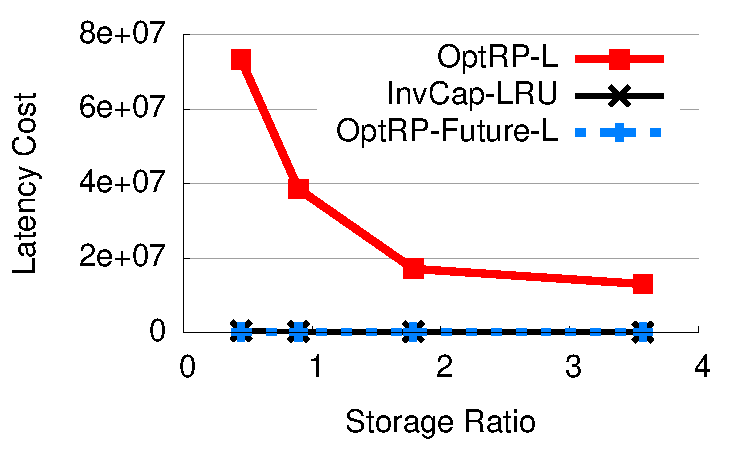
\includegraphics[scale=0.45]{graphSet1/latencycost/ATTNews.pdf}}
\subfigure[Entertainment,  US-ISP] {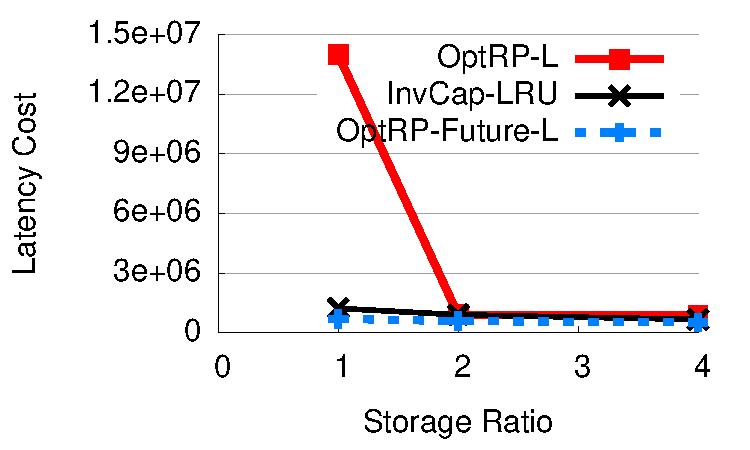
\includegraphics[scale=0.45]{graphSet1/latencycost/ATTVideos.pdf}}
\subfigure[Downloads,  US-ISP] {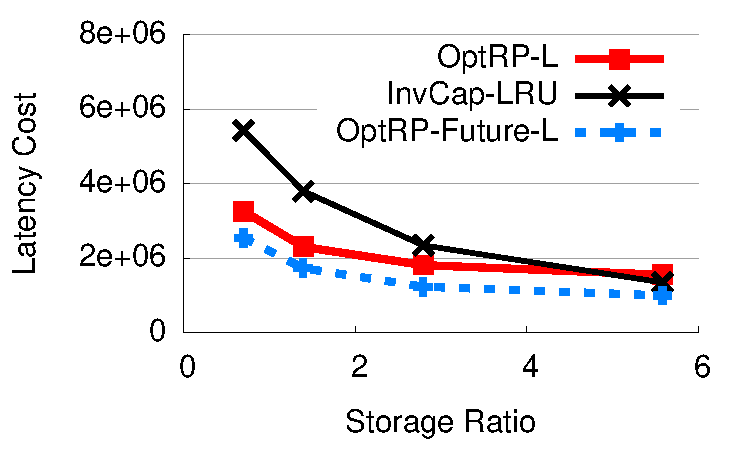
\includegraphics[scale=0.45]{graphSet1/latencycost/ATTDownloads.pdf}}
%\subfigure[News,  Abilene] {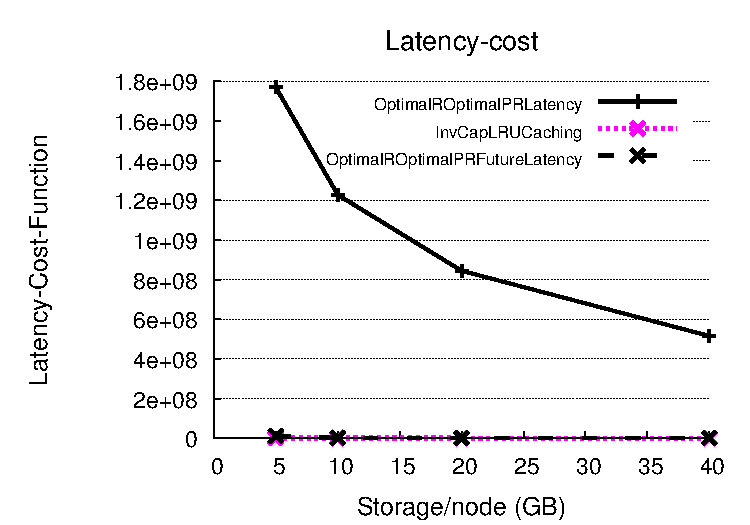
\includegraphics[scale=0.45]{graphSet1/latencycost/AbileneNews.pdf}}
%\subfigure[Entertainment,  Abilene] {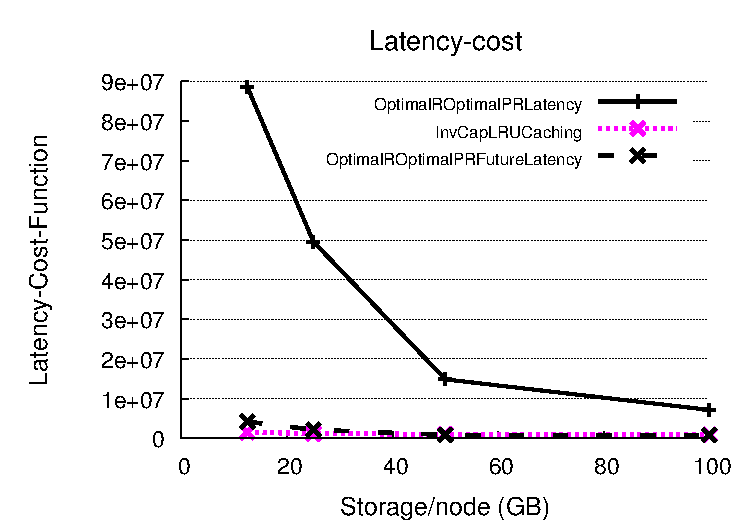
\includegraphics[scale=0.45]{graphSet1/latencycost/AbileneVideos.pdf}}
%\subfigure[Downloads,  Abilene] {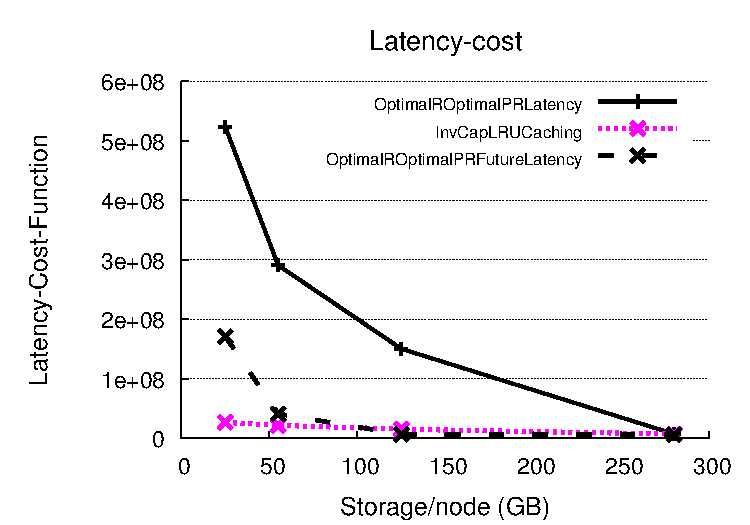
\includegraphics[scale=0.45]{graphSet1/latencycost/AbileneDownloads.pdf}}
\end{center}
\vspace{-0.2in}
\caption{ A realistic \planned\ scheme, \optrpl\ causes excessively high latency costs in some cases. \invlru\ achieves latency costs close to ideal \planned\ scheme, \optrpfuturel,  at higher storage ratios.}
\vspace{-0.2in}
\label{fig:latencygraphs}
\end{figure*}




The latency cost of \invlru\ relative to \optrpfuturel\ improves with an increase in storage ratio. At the smallest storage ratio, \invlru\  has 70-110\% higher latency cost than \optrpfuturel. The difference reduces to  14-34\% at the maximum storage ratio. Higher storage ratio translate to higher cache hit rates, which reduces propagation delay of transfers and lowers link utilizations. Both these factors contribute to  a smaller latency cost for \invlru. 
This finding shows that NCDNs can achieve close to best latency costs with a \unplanned\ scheme \invlru\ and provisioning moderate amounts of storage.

The performance of \optrpl\ on the downloads trace is much closer to \optrpfuturel\ than on the other two traces. 
Unlike other traces, content popularity is highly predictable on the downloads trace based on yesterday's demand, except for a day on which multiple new software releases were done.  On all days except one,  \optrpl\ has nearly optimal latency cost and it incurs a higher latency cost on one day of the trace. As a result, \optrpl's aggregate latency cost summed over all days is only moderately higher than that of \optrpfuturel. 



\subsection{Effect of NCDN traffic on network cost}
This experiment, unlike previous experiments, considers a network consisting of both ISP and NCDN traffic. Our goal is to evaluate how network costs change as the fraction of NCDN traffic increases in the network. Second, we seek to examine the benefit of optimizing routing over an unplanned routing scheme, InvCap. To this end, we compare the performance of \invlru\ and \optlru\ schemes. The latter scheme optimizes routing for the combined traffic matrix due to NCDN traffic and ISP transit traffic. 
In order to estimate the best gains achievable with an optimized routing, we provide to the \optlru\ scheme knowledge of future ISP traffic matrices. \optlru\ cannot be provided the knowledge of future NCDN traffic matrices because NCDN traffic matrices can only be measured from experiment itself and we do not know them beforehand. We optimize routing once a day in this experiment. Varying the frequency of routing update did not improve \optlru's performance.



We experiment with  hourly transit traffic matrices spanning 7 days from the same Tier-1 ISP --- US-ISP. These matrices were collected in February, 2005.
 Since ISP traffic volumes are much higher than NCDN traffic volumes, at first, we performed this experiment by scaling down the ISP traffic matrices, so that ISP and NCDN traffic have comparable volumes. Of the total NCDN traffic, less than 10\%  reaches the backbone links, rest is served locally by PoPs. 
For equal volumes of NCDN and ISP traffic we expected the MLU of a network  with ISP traffic only to be much higher than MLU for the network with only NCDN traffic. 
Our experiment showed that MLU for ISP traffic and NCDN traffic are nearly the same.

We found that this was because the NCDN traffic showed highly variable link utilization even over the course of a few minutes: the maximum link utilization differed by up to 3$\times$  in the course of 15 minutes. The hourly ISP traffic matrix that we experimented with  retained the same, smoothed utilization level for an hour.  As a result, 99-percentile MLU's for NCDN traffic are the same as that for ISP even though its aggregate backbone traffic was much lesser.


To make the variability of NCDN traffic comparable to ISP traffic, we scaled up the volume of NCDN traffic. The scaling is done by introducing new content similar to a randomly chosen content in the original trace. 
Each new content is of the same size, and same video bit rate  as the original content. All requests for the new content are made from the same locations, at approximately the same times (within an 1-hour window of the request of the original content),  and are of the same durations as the requests for the original content. Our scaling preserves the popularity distribution of objects and the geographic and temporal distribution of requests. We scaled our trace to the maximum level so as to not exceed the memory available (8 GB) in our machine.


\begin{figure}
\begin{center}
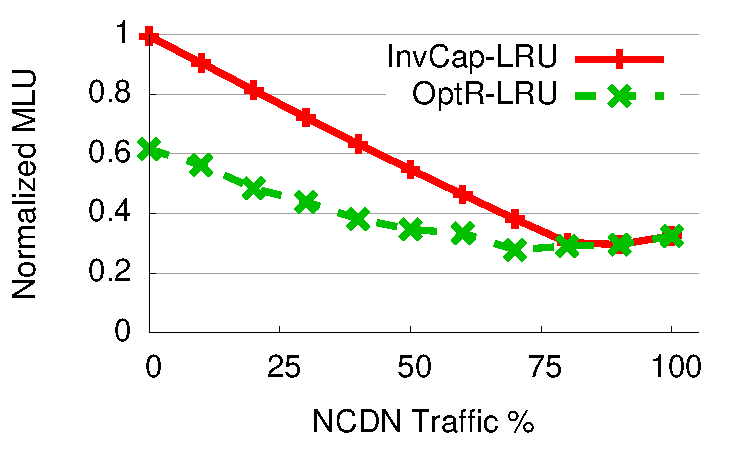
\includegraphics[scale=0.4]{graphset1/ispncdn/ATTNews-99percentile.pdf}
\vspace{-0.25in}
\end{center}
\caption{[News, US-ISP]Network costs at varying fractions of NCDN traffic in an ISP network.}
\label{fig:ispncdn}
\vspace{-0.2in}
\end{figure}

We present the results of our experiments on the news trace in Figure \ref{fig:ispncdn}. We vary the fraction of NCDN to ISP traffic, and report MLUs normalized by the total volume of ISP and NCDN traffic.
Our results are not independent of the scale of simulations: a larger or a smaller scaling of CDN trace may give quantitatively different conclusions. Hence, we only make qualitative conclusions from this experiment. First, we find that as the fraction of NCDN traffic increases, MLU decreases for both schemes. This is intuitive since a large fraction of NCDN traffic is served from caches located at PoPs. Second, as NCDN traffic increases optimizing routing (\optlru) gives lesser benefits compared to InvCap routing.  In a network dominated by NCDN traffic, optimizing routing gives almost no benefits over \invlru. We find these results to be consistent with our earlier experiments with NCDN traffic only.

%Our results depend on the scale at which we do our experiments. Therefore, we can only qualitative conclusions from this experiments. 
%We find that as the fraction of NCDN traffic increases MLU decreases for both schemes. This is intuitive as more and more NCDN traffic is cached inside the network which reduces MLU for both schemes.
%As NCDN traffic optimizing routing gives small benefits compared to \optlru. 
%In a network dominated by NCDN traffic, optimizing routing gives almost no benefits over \invlru.

%We present the results of our experiments on the News trace in Figure \ref{fig:ispncdn}. 
%We vary the fraction of NCDN traffic and we compare both ISP and NCDN traffic in the network. 
%We compare the performance of two schemes \invlru\ and \optrp. \optrp\ optimizes the combined traffic matrix due to NCDN traffic and ISP transit traffic matrix.
%

%We provide the benefit of future knowledge of ISP transit traffic matrix to \optlru\ to estimate the best network costs that optimizing routing can achieve. 
%
%We vary the frequency of optimizing routing which ISP can 
%
%Optimizing routing gives benefits relative to InvCap.
%
%Difference reduces as fraction of NCDN traffic increases. 




%\textbf{A note on the need for traffic engineering:} Overall, our results suggest that optimizing routing yields little improvement to network cost for the NCDN portion of the traffic, but this finding does not imply that traffic engineering by ISPs is unnecessary. ISPs route transit traffic in addition to NCDN traffic, and they do not control either content placement or request redirection for transit traffic, therefore, traditional traffic engineering methods, e.g., OSPF traffic engineering, can reduce the network cost due to transit traffic. The benefit of traffic engineering, or lack thereof, depends on the fraction of transit traffic vs. NCDN traffic in an ISP.


\eat
{

\subsection{Is Traffic Engineering Irrelevant?}

\textbf{Transit traffic:} Optimizing routing gives little improvement to network cost in an NCDN but this finding does not obviate traffic engineering by ISPs.  The primary reason ISPs need traffic engineering is that they route transit traffic in addition to NCDN traffic. Since an ISP does not control either content placement or request redirection for transit traffic, traditional traffic engineering methods, e.g., OSPF traffic engineering, can reduce the network cost due to transit traffic.

\textbf{Link failures:} Minimizing network cost in case of link failures is another objective of traffic engineering. Therefore, we evaluate performance of \invlru\ and \optrpfuture\  in case of all single link failures. We compare these schemes based on the highest network cost across all failures. For this experiment, we added a constraint to the MIP in Section \ref{sec:linearprograms} which ensures that \optrpfuture\ is resilient to any single link failure. The complete description of this constraint is presented in \cite{techreport}.


In Figure  \ref{fig:linkfailurecompare}, we show the network cost of \invlru\ and \optrpfuture\ in failure-free scenario and their network costs during failures. Both \invlru\ and \optrpfuture\ see up to 110\% and 99\% increase in network cost  respectively during failures. During failures we find that \invlru\  has a significantly higher network cost than \optrpfuture\  at small storage ratios, but the difference reduces at higher storage ratios with \invlru\ even achieving a lower network cost than \optrpfuture\ at the maximum storage ratio in each graph.  Comparing the failure-free scenario and link failure scenarios, the relative sub-optimality of \invlru\ with respect to \optrpfuture\ remains the same at small storage ratios or but reduces at higher storage ratios. 
%The nonmonotonicity of \optrpfuture\ is because it optimizes routing and placement assuming a failure-free scenario and hence performs sub-optimally when link failures occur.

\begin{figure}
\begin{center}
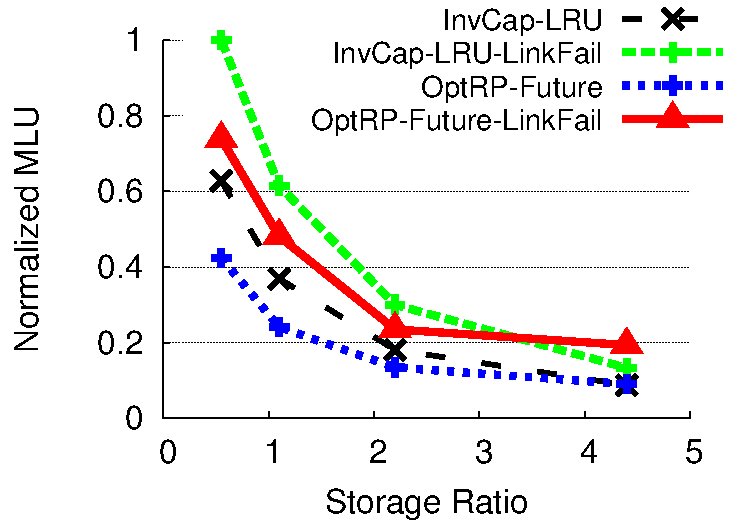
\includegraphics[scale=0.45]{graphSet1/linkfailurecompare/AbileneVideos.pdf}
\end{center}
\vspace{-0.25in}
\caption{During link failures, \invlru\ can achieve a lower network cost than \optrpfuture\ at high storage ratios. Entertainment trace, Abilene}
\vspace{-0.2in}
\label{fig:linkfailurecompare}
\end{figure}

}

\subsection{Other Results and Implications}
\label{sec:additional}
%We summarize our main conclusions from the rest of our experiments here and refer the reader to \cite{techreport} for a complete description of these experiments:

We summarize our findings from  other experiments with NCDN traffic here due to space constraints.
%and refer the reader to \cite{techreport} for a full description.

{\bf Link-utilization aware redirection:}
We evaluate a request redirection strategy for \invlru\ that periodically measures link utilizations in the network and prefers less loaded paths while redirecting requests.
Our evaluation shows that such a redirection gives small benefits in terms of network cost ($7\%-13\%$) and gives almost no benefits on latency costs. 
This implies that sophisticated network-aware redirection strategies  may be of little value for an NCDN. 

\textbf{Request redirection to neighbors:}  If each PoP redirects requests only to its one-hop neighbor PoPs before redirecting to the origin, \invlru\ incurs only a moderate (6\%-27\%) increase in the MLU. However, if a PoP redirects to no other PoPs but redirects only to the origin, the MLU  for \invlru\ increases significantly (25\%-100\%). Thus, request redirection to other PoPs helps reduce network cost, but most of this reduction can be had by redirecting only to neighboring PoPs.
%\textbf{Request redirection to neighbors:}  If each PoP redirects requests only to its one-hop neighbor PoPs before redirecting to the origin, \invlru\ incurs only a moderate (6\%-27\%) increase in the MLU. However, if a PoP redirects to no other PoPs but redirects only to the origin, the MLU  increases significantly (25\%-100\%). Thus, request redirection to other PoPs helps reduce network cost, but most of this reduction can be had by redirecting requests only to neighboring PoPs.

%Thus, \invlru\ can get most of the benefits of  redirection to other PoPs  by redirecting  only to the neighboring PoPs.

\textbf{Heterogenous storage:} Heterogenous storage at PoPs  (storage proportional to the number of requests at a PoP in a trace, and other simple heuristics) increases the MLU compared to homogenous storage for both \invlru\ and \optrpfuture, and makes \invlru\ more sub-optimal compared to \optrpfuture. This leads us to conclude that our results above with homogeneous storage are more relevant to practical settings.

%This suggests that an NCDN should provision storage homogeneously at PoPs.
%

%  Varying the frequency at which \optlru\ updates routing in the range of 3 hours (default) to 24 hours

\textbf{\optlru\ parameters:} Whether \optlru\ updates routing every 3 (default), 6, or 24 hours,  makes little difference to its performance. Further, whether \optlru\  optimizes routing using traffic matrix measured over the immediately preceding three hours (default) or using traffic matrices measured the previous day, its network cost remains nearly unchanged. These experiments reinforce our finding that optimizing routing gives minimal improvement over \invlru.

%Whether \optlru\ updates routing every 3 hrs (default), 6 hrs, or 24 hrs,  makes little difference to its performance. Further, whether \optlru\  optimizes routing using traffic matrix measured over the immediately preceding three hours (default) or using traffic matrices measured the previous day, its network cost remains nearly unchanged. These experiments reinforce our finding that optimizing routing gives minimal improvement over \invlru. 
\textbf{Number of exit nodes:} When the number of network exit nodes is increased to five or decreased to one, our findings in Section \ref{sec:videodownload} remain qualitatively unchanged.
%\textbf{Exit nodes:} Even when the network has one exit node or five exit nodes connected to the origin, instead of three, our main findings in Section \ref{sec:videodownload} still hold true.
%Whether the number of exit nodes connected to the origin is one, or three (default value), or five, . 
%Even when the number of exit nodes connected to the origin is  reduced from three (default) to one, or increased from three to five, our main findings from the prior sections still hold true. 



%If each PoP redirects requests only to its one-hop neighbor PoPs on a cache miss before redirecting to the origin, \invlru\ incurs only a moderate (25\%) increase in MLU. However, if a PoP contacts no other PoPs on a cache miss but directly contacts the origin, MLU for \invlru\  increases by up to 100\%. So, \invlru\  need    redirecting requests to a small subset of PoPs brings significant MLU reduction. 

\textbf{Link failures:} The worst-case network cost across all single link failures for \invlru\ as well as \optrpfuture\ is approximately twice compared to their network costs during  a failure-free scenario. Comparing the failure-free scenario and link failure scenarios, the relative sub-optimality of \invlru\ with respect to \optrpfuture\ remains the same at small storage ratios but reduces at higher  ratios. 


\subsection{Limitations}

Although we have evaluated several NCDN management strategies, our experimental methodology suffers from some shortcomings. First, we assume that servers deployed at each PoP have enough resources to serve users requests for locally cached content.  In cases when server resources are inadequate, e.g., due to flash crowds, a simple redirection strategy, e.g.,  redirection to the closest hop-count server used by the \invlru\ scheme, may result in poor user-perceived performance. In practice, NCDNs should adopt a redirection strategy that takes  server load into account to handle variability of user demands.  Second, we model user-perceived latency using a latency cost function that considers propagation delays and link utilization levels. Our latency cost function is a crude approximation of user-perceived latency.  A  better metric would be based on the TCP throughput experienced by a user. However, an accurate estimation of TCP throughputs of users at the scale of an ISP network with dynamic workloads is extremely challenging. We defer addressing these concerns to future work.



\eat{
\begin{itemize}
\item Heterogenous storage at PoPs  (storage proportional to average number of requests at a PoP) increases the MLU compared to homogenous storage for both \invlru\ and \optrpfuture, but makes \invlru\ more sub-optimal compared to \optrpfuture.
\item Varying the frequency at which \optlru\ updates routing in the range of 3 hours (default) to 24 hours make little difference to its performance. Further, whether routing is optimized using traffic matrix measured over the immediately preceding three hours (default) or traffic matrices measured the previous day, network cost remains unchanged. 
\item Even when the number of exit nodes connected to the origin is  reduced from three (default) to one, or increased from three to five, our main findings from the prior sections still hold true. 
\item If each PoP redirects requests only to its one-hop neighbor PoPs on a cache miss before redirecting to the origin, \invlru\ incurs only a moderate (25\%) increase in MLU. However, if a PoP contacts no other PoPs on a cache miss but directly contacts the origin, MLU for \invlru\  increases by up to 100\%. So, \invlru\  need    redirecting requests to a small subset of PoPs brings significant MLU reduction. 
\end{itemize}
}

